\fancyhead[L]{\fontsize{9pt}{11pt}\selectfont\textbf{\textsf{8}}\qquad \textbf{\textsf{CHƯƠNG 1}}\quad \textsf{Các hàm số và Mô hình}}
\fancyhead[R]{}

\noindent
\begin{minipage}[t]{0.268\textwidth}
    % 4 vạch cyan trên cùng bên lề
    \vspace*{-2pt}%
    {\color{stewartcyan}%
    \rule{\linewidth}{0.5pt}\vspace{3.5pt}\par
    \rule{\linewidth}{0.5pt}\vspace{3.5pt}\par
    \rule{\linewidth}{0.5pt}\vspace{3.5pt}\par
    \rule{\linewidth}{0.5pt}\par
    }

    \vspace{1.15cm}
    \noindent
    {\fontsize{9pt}{11pt}\selectfont\textbf{\textsf{Bảng 1}}\quad \textsf{Dân số thế giới}}\\[2pt]
    {\fontsize{8pt}{9.8pt}\selectfont
    \setlength{\tabcolsep}{4pt}
    \renewcommand{\arraystretch}{1.08}
    \begin{tabular}{|c|c|}
        \hline
        \rowcolor{stewarttableheader}
        \textbf{Năm} & \textbf{\makecell{Dân số\\(triệu người)}} \\
        \hline
        1900 & 1650 \\
        1910 & 1750 \\
        1920 & 1860 \\
        1930 & 2070 \\
        1940 & 2300 \\
        1950 & 2560 \\
        1960 & 3040 \\
        1970 & 3710 \\
        1980 & 4450 \\
        1990 & 5280 \\
        2000 & 6080 \\
        2010 & 6870 \\
        \hline
    \end{tabular}}

    \vspace{3.0cm}
    {\raggedleft
    {\fontsize{9pt}{11pt}\selectfont\textbf{\textsf{HÌNH 1}}}\\[2pt]
    {\fontsize{7.8pt}{9.8pt}\selectfont\color{darkgray} Gia tốc mặt đất theo phương thẳng đứng\\trong trận động đất Northridge}\par}
\end{minipage}%
\hfill
\begin{minipage}[t]{0.705\textwidth}
    \vspace*{-8pt}
    \noindent
    {\color{stewartcyan}\fontsize{15pt}{18pt}\selectfont\textbf{\textsf{1.1}}}%
    \hspace{6pt}%
    {\color{stewartcyan}\rule[-2pt]{0.8pt}{14pt}}%
    \hspace{6pt}%
    {\fontsize{15pt}{18pt}\selectfont\textbf{\textsf{Bốn cách biểu diễn một hàm số}}}
    
    \vspace{8pt}
    \noindent{\fontsize{10.5pt}{13pt}\selectfont\textbf{\textsf{\color{stewartcyan}■ Các hàm số}}}
    \vspace{3pt}

    Hàm số xuất hiện bất cứ khi nào một đại lượng này phụ thuộc vào một đại lượng khác. Hãy xem xét bốn tình huống sau:

    \begin{enumerate}[label=\textbf{\Alph*.}, leftmargin=1.5em, itemsep=1.5pt, topsep=2pt, parsep=0pt]
        \item Diện tích $A$ của một hình tròn phụ thuộc vào bán kính $r$ của hình tròn đó. Mối liên hệ giữa $r$ và $A$ được xác định bởi công thức $A = \pi r^2$. Ứng với mỗi số dương $r$, ta luôn xác định được duy nhất một giá trị $A$ tương ứng, và ta nói rằng $A$ là một \textit{hàm số} của $r$.

        \item Dân số thế giới $P$ phụ thuộc vào thời gian $t$. Bảng 1 cung cấp số liệu ước tính về dân số thế giới $P$ tại các mốc thời gian $t$ trong một số năm nhất định. Chẳng hạn:
        \[
        P \approx 2{,}560{,}000{,}000 \quad \text{khi } t = 1950
        \]
        Ứng với mỗi giá trị của thời gian $t$, luôn có một giá trị tương ứng của $P$, và ta nói rằng $P$ là một hàm số của $t$.

        \item Cước phí bưu điện $C$ để gửi một phong bì phụ thuộc vào khối lượng $w$ của nó. Dù không có một công thức toán học đơn giản nào biểu diễn trực tiếp mối quan hệ giữa $w$ và $C$, bưu điện vẫn có một bảng quy tắc rõ ràng để xác định giá trị của $C$ khi biết trước $w$.

        \item Gia tốc thẳng đứng $a$ của mặt đất đo được bởi một địa chấn kế trong suốt một trận động đất là một hàm số theo thời gian trôi qua $t$. Hình 1 thể hiện đồ thị ghi lại hoạt động địa chấn trong trận động đất Northridge làm rung chuyển Los Angeles vào năm 1994. Với một giá trị thời gian $t$ cho trước, đồ thị cung cấp cho ta một giá trị gia tốc $a$ tương ứng.
    \end{enumerate}

    \vspace{2pt}
    {\centering
    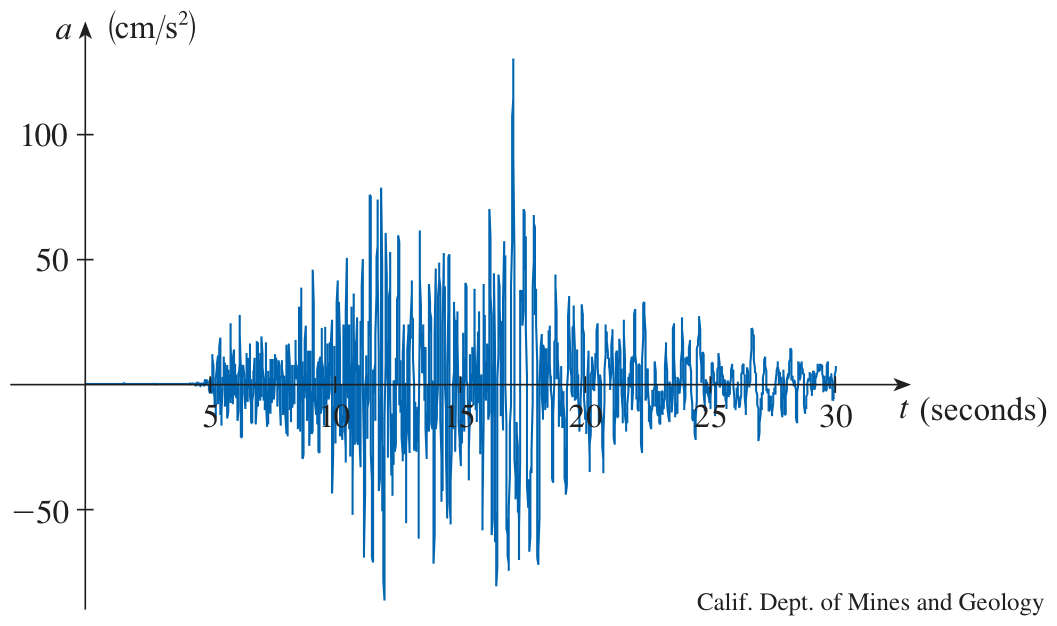
\includegraphics[width=7.6cm]{images/figure_1_tight.png}\par}
    \vspace{2pt}

    Mỗi ví dụ trên đều mô tả một quy tắc sao cho khi cho trước một số ($r$ trong Ví dụ A), một giá trị số khác ($A$) sẽ được xác định tương ứng. Trong mỗi trường hợp, ta nói rằng số thứ hai là một hàm số của số thứ nhất. Nếu dùng chữ cái $f$ để đại diện cho quy tắc liên hệ giữa $A$ và $r$ trong Ví dụ A, ta biểu diễn mối liên hệ này bằng \textbf{ký hiệu hàm số} là $A = f(r)$.

    \vspace{4pt}
    \begin{definitionbox}
    Một \textbf{hàm số} $f$ là một quy tắc đặt tương ứng mỗi phần tử $x$ thuộc một tập hợp $D$ với duy nhất một phần tử, ký hiệu là $f(x)$, thuộc một tập hợp $E$.
    \end{definitionbox}

    \vspace{4pt}
    \noindent
    Chúng ta thường khảo sát các hàm số mà các tập hợp $D$ và $E$ đều là tập hợp các số thực. Tập hợp $D$ được gọi là \textbf{tập xác định} (\textit{domain}) của hàm số. Số $f(x)$ được gọi là \textbf{giá trị của $f$ tại $x$} và được đọc là ``$f$ của $x$'' (hay ``$f$ tại $x$''). \textbf{Tập giá trị} (\textit{range}) của $f$ là tập hợp tất cả các giá trị có thể có của $f(x)$ khi $x$ biến thiên trên toàn bộ tập xác định.
\end{minipage}